\pagestyle{fancy}
\lhead{}
\renewcommand{\chaptermark}[1]{\markboth{\thechapter.\ #1}{}}
\chapter{Experimental measurement techniques}
\label{ch:experimentalSetups}

In this thesis we used several experimental techniques:

\begin{itemize}
  \item An optical switching experiment based on controlling a low-power signal (probe) through high power pulses (pump).
  \item Phase and amplitude measurements of Kerr, TPA and carrier response with high temporal resolution, using phase-sensitive time resolved measurements.
  \item Four wave mixing experiment to measure the nonlinear coefficient ($Re\{\gamma\}$).
  \item TPA estimation from pulsed transmission to measure the nonlinear loss coefficient ($Im\{\gamma\}$). From the nonlinear coefficient ($Re\{\gamma\}$) and loss ($Im\{\gamma\}$) we can calculate the nonlinear figure of merit.
  \item Phase sensitive measurements to obtain dispersion, group index and phase spectrum.
  \item Optical vector analyzer to measure amplitude and phase response.
\end{itemize}

\section{All optical switching}
\label{ch:allOpticalSwitching}
Fig.~\ref{fig:switchingSetupSwitching} shows the setup for the all-optical switching experiment.
We use a 40~Gb/s bit pattern generator to generate short and low repetition pulses that drive an external $ \mathrm{LiNbO_3} $ modulator.
After modulating the signal of the tunable laser we amplify the pump pulses using Er-doped fiber amplifiers (EDFAs).
Then, the pump is mixed with a continuous-wave (CW) probe signal using a 3~dB coupler and sent to the sample through the same fiber.
We choose pump and probe wavelengths to match with two resonances of a micro-ring resonator.
Finally, the output signal is filtered to remove the pump component and amplified before sending the signal to the photodiode of a sampling scope that collects the data.

\begin{figure}[htb]
    \centering
    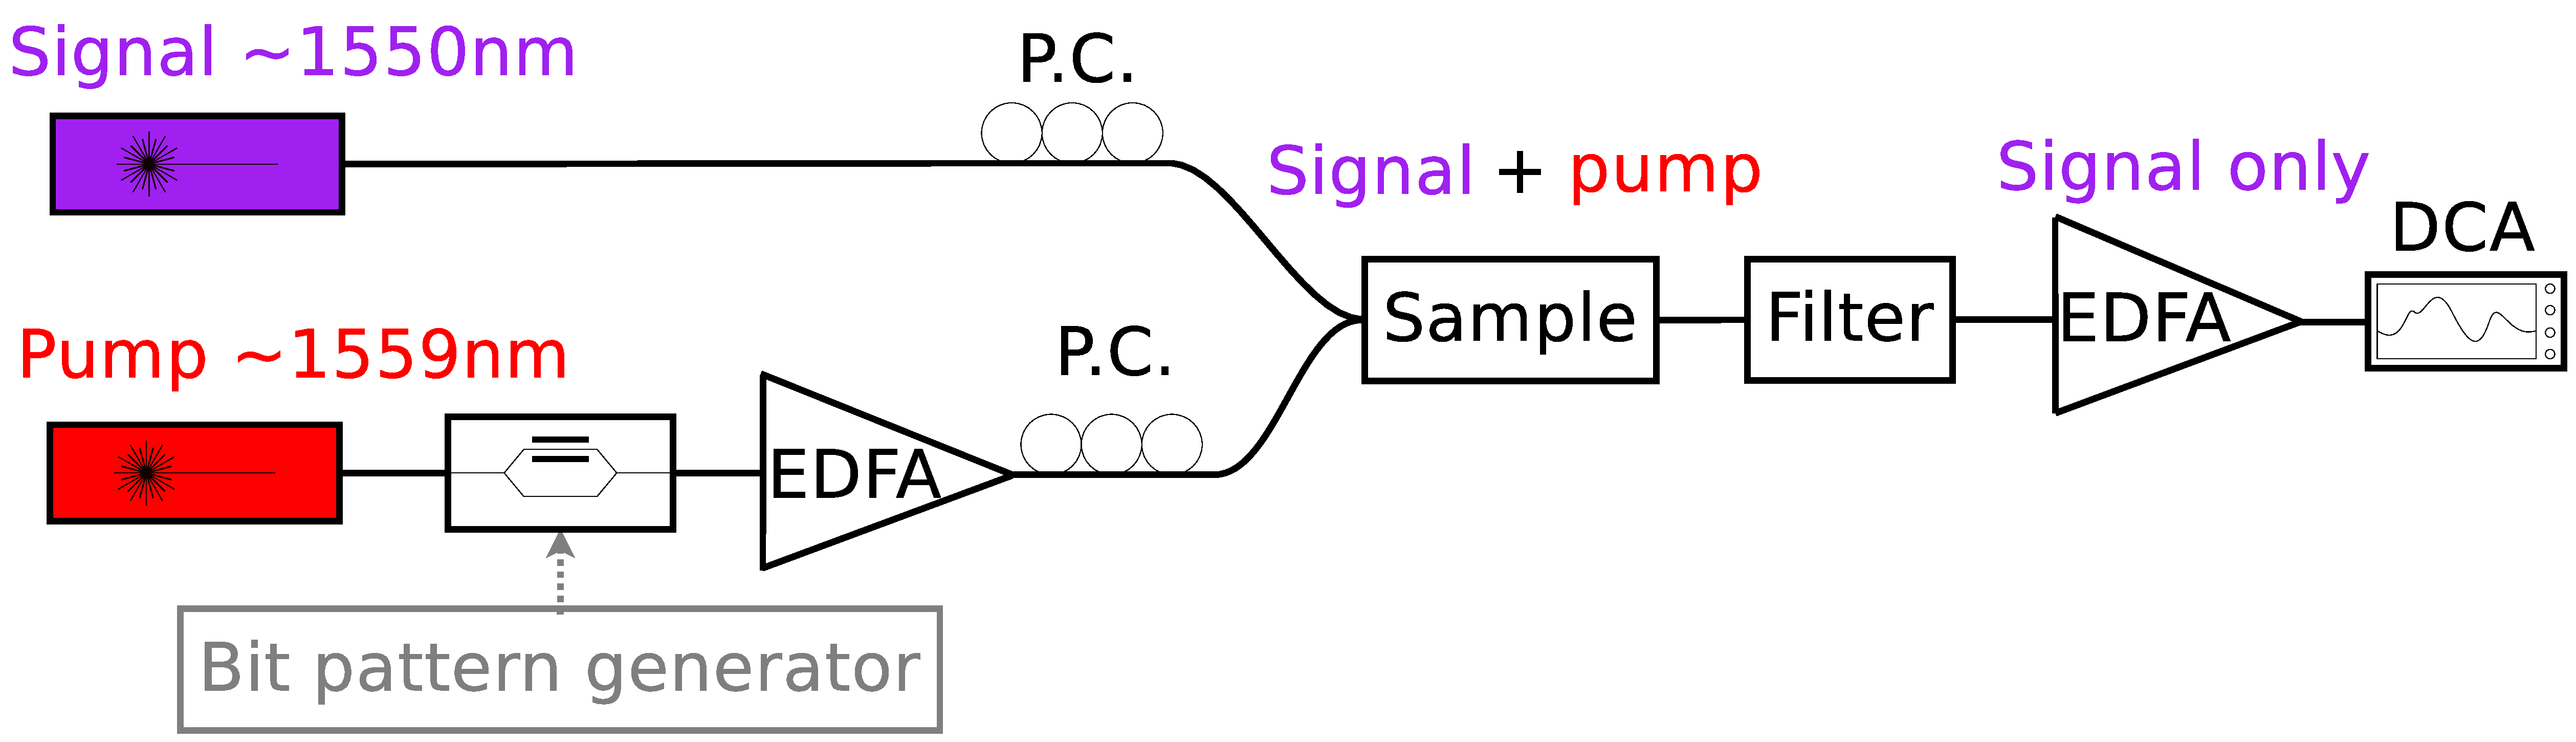
\includegraphics[width=1.0\textwidth]{switching}
    \caption{All-optical switching characterization setup. (Triangles represent EDFAs with ASE filters, PC: polarization controllers, DCA: Digital communication analyzer)}
    \label{fig:switchingSetupSwitching}
\end{figure}

% 
% \begin{figure}[htb]
%     \centering
%     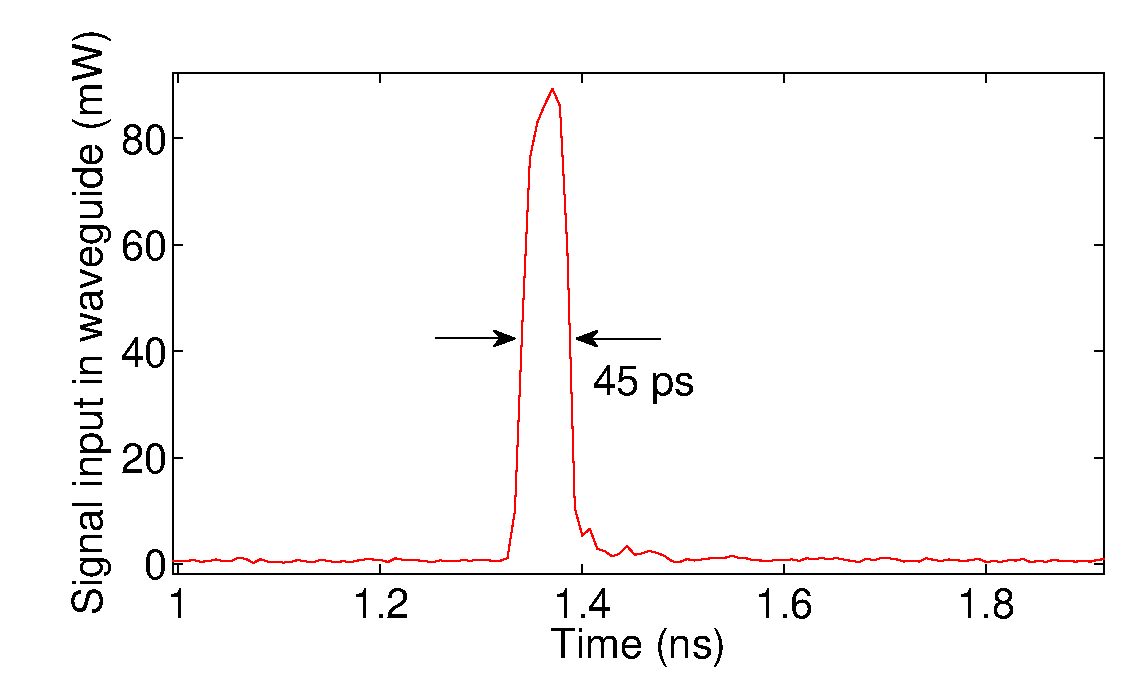
\includegraphics[width=0.49\textwidth]{inputPulsesSwitchingBig}
%         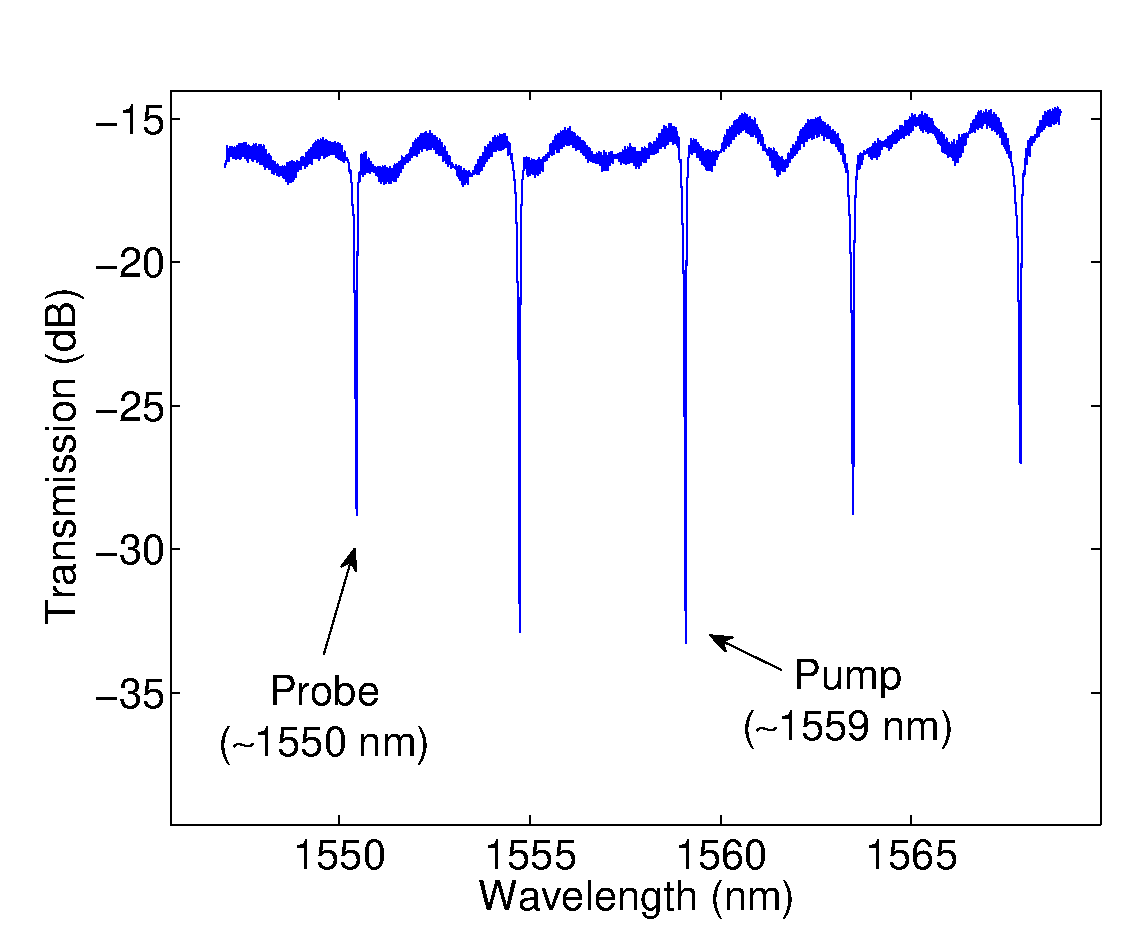
\includegraphics[width=0.49\textwidth]{broadBig}
%     \caption{Left: Input pulses with 45~ps duration, 6.4~ns period and 85~mW peak power coupled in the waveguide. 
%     Right: Transmission spectrum of the ring resonator sample (TM polarization). Wavelengths of pump and probe signals were respectively 1559 and 1550~nm.}
%     \label{fig:inputPulsesSwitchingBig}
% \end{figure}
% 
% Figure \ref{fig:ntc02switching} shows the result of the all-optical switching experiment in silicon micro-ring resonators~\cite{Oton,optoel}. The carrier dispersion effect produces a phase response, which is converted into intensity modulation by using a micro-ring resonator. The resonance position blue-shifts when the carriers are excited, so with the probe tuned to the resonance this shift produces an intensity modulation. Using 85~mW of pump peak power, the extinction ratio is 10.2~dB and the 1/e recovery time is 150~ps. Depending on which point of the resonances we tune our CW laser we can obtain positive (laser in the minimum of the resonance) or negative pulses (CW laser next to the resonance). 
% 
% \begin{figure}[htb]
%     \centering
%     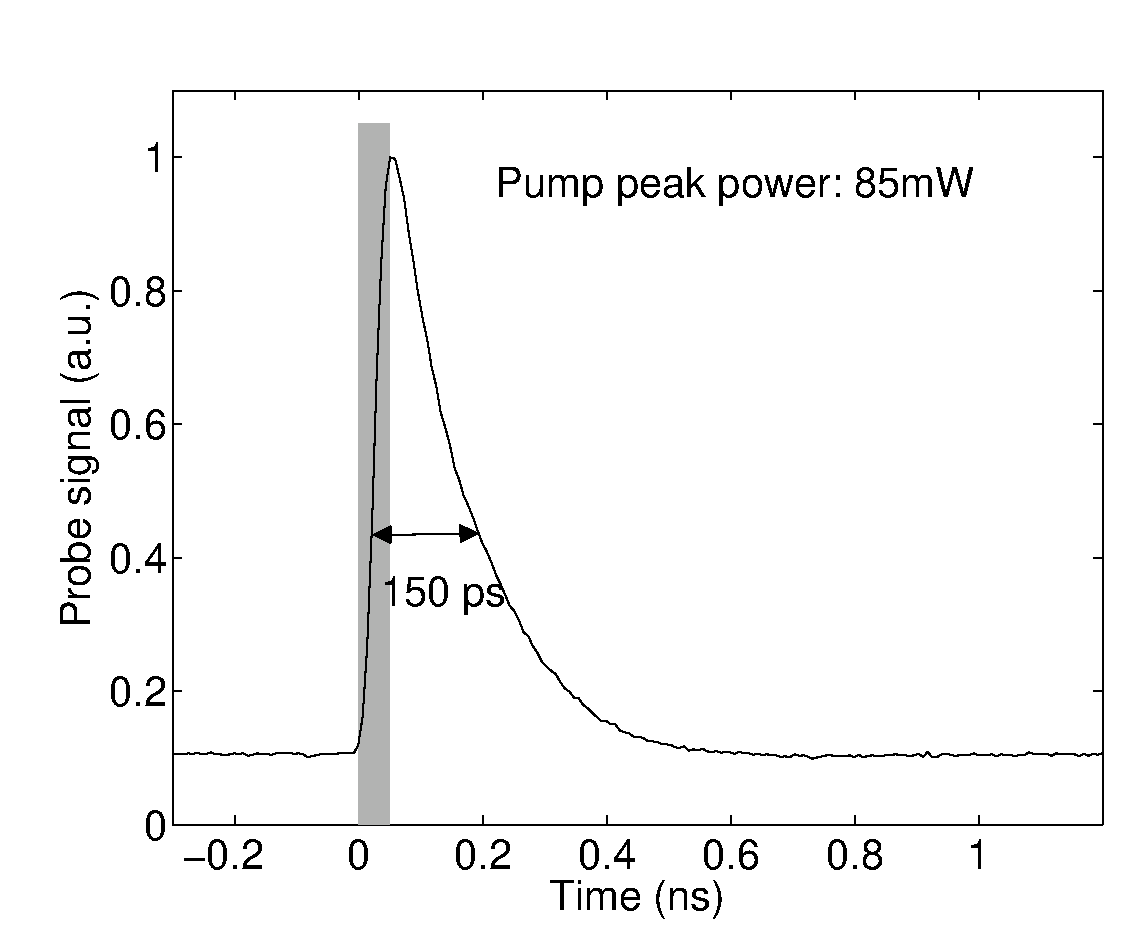
\includegraphics[width=0.49\textwidth]{pos_pulse_big}
%     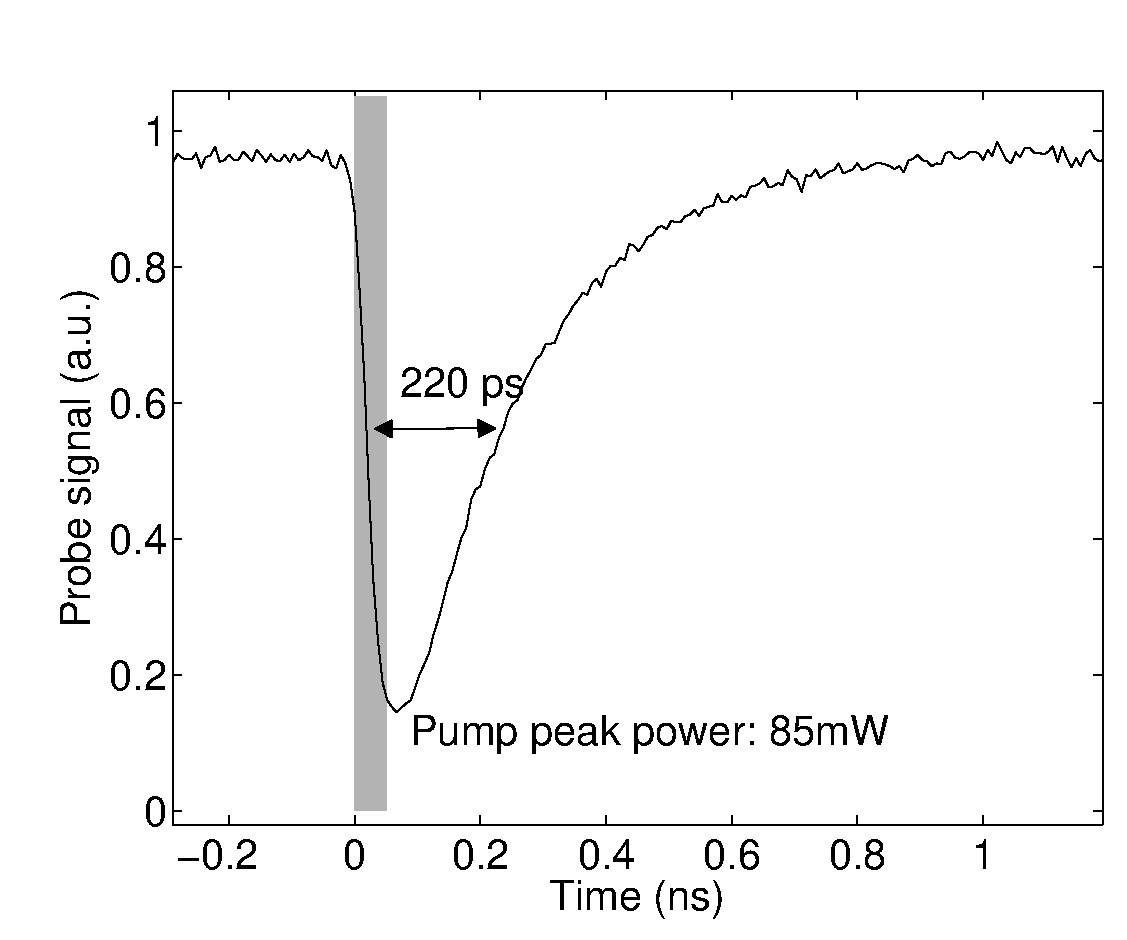
\includegraphics[width=0.49\textwidth]{neg_pulse_big}
%     \caption{Variation of the probe signal when both pump and probe are resonant with two different modes of the microring. The grey box marks the pump duration. Depending on which point of the resonances we tune our CW laser we obtain positive (left figure) or negative pulses (right figure).}
%     \label{fig:ntc02switching}
% \end{figure}

\section{Phase-sensitive nonlinear time resolved measurements}
\label{ch:timeRes}
In order to study in with great detail the nonlinear effects dynamics, both in phase and module, we used an heterodyne characterization setup. The set up (Fig.~\ref{fig:timeResSetupTesis}) consists of a series of probe pulses that are affected by a high power pulses (pump). Varying the pump pulses with respect to the probe ones we can see the module and phase response of nonlinear effects such as Kerr, cross absorption modulation, Free-carrier absorption and Free-carrier dispersion.

\begin{figure}[htb]
    \centering
    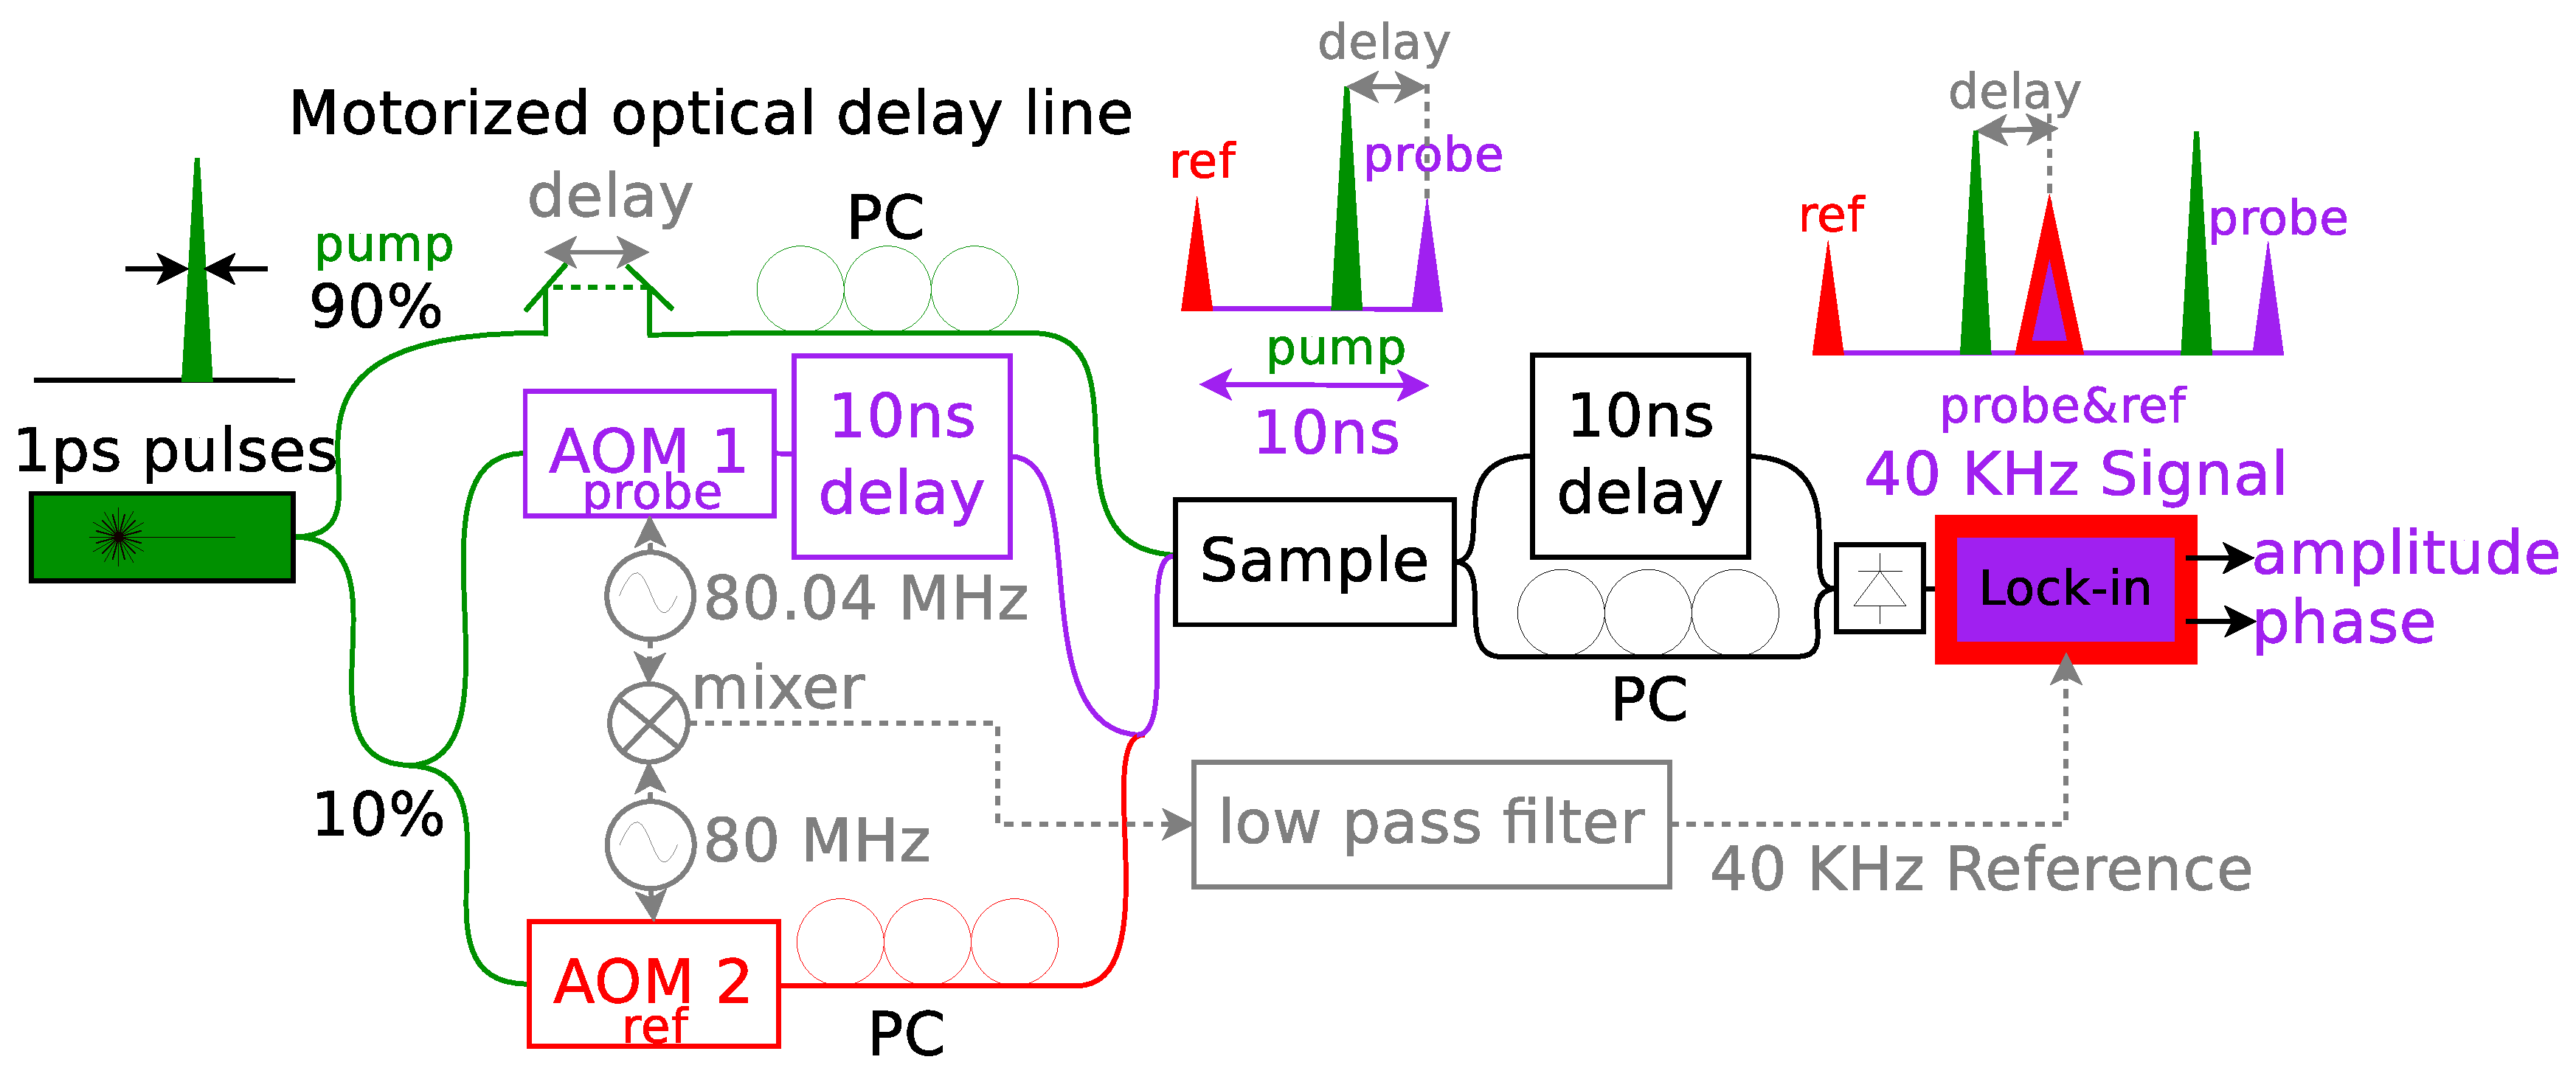
\includegraphics[width=1.0\textwidth]{timeResolvedBig}
    \caption{The lock-in detects the phase and the amplitude of the 40~kHz probe and reference beatings. Measuring the changes of the pump in the probe for different delays between them. PC: polarization controller. }
    \label{fig:timeResSetupTesis}
\end{figure}

The initial pulse is divided into three pulses: two weak ones (a reference and probe separated 10~ns), and one pump pulse, situated close to the probe pulse, and whose temporal position with respect to the probe can be varied. The reference and probe pulses are recombined after passing through the sample, and the beatings they produce are collected in the lock-in. The 40~KHz beatings  are produced because the wavelengths of probe and reference signals are slightly different, as both are shifted with acousto-optic modulators which work at frequencies that only differ by 40~kHz. The amplitude and the phase of the signals are simultaneously monitored.
The amplitude collected is proportional to the amplitude of the probe pulse with respect to the reference, and the phase of the beatings corresponds to the phase shift produced by the pump to the probe pulse, considering the reference pulse as unaffected by the pump, and thus using it as a reference for the phase measurement. 

The phase drift observed required a special way of acquiring the data, referencing every time at a fixed delay, in order to compensate for the phase drift.

\section{Four wave mixing}
\label{ch:fwm}
Four wave mixing measurements are very useful to extract the nonlinear coefficient ($\gamma$) and dispersion (D) of integrated waveguides.
We boost two laser signals and filter the ASE from the EDFAs using bandpass filters.
To inject the correct polarization into the chip we use independent polarization controllers (Fig.~ \ref{setup}).
Finally, we fix the wavelength of a high power $Pump$ and measure the conversion efficiency for different $Signal$ wavelengths.  


\begin{figure}[htb]
	\centering
	\includegraphics[width=1.00\textwidth]{fwm}
	\captionof{figure}{Four Wave Mixing characterization setup. PC: polarization controllers, OSA: optical spectrum analyzer.}
	\label{setup}
\end{figure}

FWM conversion efficiency is defined as the power ratio between generated idler and signal ($P_i/P_s$).
The bandwidth of the conversion efficiency ($\eta$) is limited by the phase mismatch between pump and signal, which depends on the dispersion (D) and pump-signal detuning ($\Delta \lambda$) ($ \eta_{\Delta\lambda \to 0,D \to 0} = 1 $)~\cite{Vallaitis2009}.


\begin{equation}
	P_i(L)=e^{-\alpha_0L}(\eta Re\{\gamma\}P_P(0)L_{eff})^2 P_s(0)
\end{equation}

\begin{equation}
	\frac{P_i(L)}{P_s(L)}=(\eta Re\{\gamma\}P_P(0)L_{eff})^2 
\label{eq:ratio}
\end{equation}

where $ L_{eff} $ is the effective waveguide length

\begin{equation}
	L_{eff}=\frac{1-e^{-\alpha_0L}}{\alpha_0}
\end{equation}

and the FWM efficiency $ \eta $:

\begin{equation}
	\eta ^2=\frac{\alpha_0^2}{\alpha_0^2+\Delta \beta^2}\left( 1+ 4e^{-\alpha_0L}\frac{sin^2(L\Delta\beta/2)}{1-e^{-\alpha_0L}} \right)
\end{equation}

where the phase mismatch for a detuning $ \Delta\lambda = \lambda_p-\lambda_s$ is:

\begin{equation}
	\Delta \beta=\frac{2\pi cD_2}{\lambda_p^2}\Delta\lambda^2
\end{equation}



\section{TPA estimation from pulsed transmission}
\label{ch:imGamma}
Two-photon absorption is a well-known process in silicon waveguides.
In a waveguide, we can consider it as the imaginary part of the gamma coefficient:

\begin{equation}
 \frac{dP}{dz} = -\alpha P(z) - 2|Im(\gamma)| P(z)^2 
\label{eq:differentialTPAImGamma}
\end{equation}

where $\alpha$ and $Im(\gamma)$ are the linear and nonlinear loss and P is the power of the signal through the waveguide.
This equation has an analytic solution \cite{Koos2007,Tsang1991}, which can be written as:

\begin{equation}
 P(L) = \frac{e^{-\alpha L}}{1+2|Im(\gamma)| L_{eff} P_0} P_0
\end{equation}

where $P_0$ is the input power in the waveguide and $L_{eff}$ is defined as:

\begin{equation}
 L_{eff} = \frac{1-e^{-\alpha_0L}}{\alpha_0}
\end{equation}


This means that the inverse of the transmission has the contribution of the nonlinear loss in the numerator and linear loss in the denominator:
\begin{equation}
 T^{-1} = \frac{P_0}{P(L)} = \frac{1+2|Im(\gamma)| L_{eff} P_0}{e^{-\alpha L}}
\end{equation}

Therefore the relationship between the low power transmission  ($T_{LP} = e^{-\alpha L} $) and high power transmission ($T_{HP} = P(L)/P_0 $) is the nonlinear loss ($T^{-1}_{NL}$):

\begin{equation}
 T^{-1}_{NL} = \frac{T_{LP}}{T_{HP}} = 1+2|Im(\gamma)| L_{eff} P_0
\label{eq:transmissionLinearImGamma}
\end{equation}

Which is a linear function on $P_0$.
The slope of the curve can give us the nonlinear loss coefficient ($Im(\gamma)$) of the waveguide as in~\cite{Vallaitis2009}.
However, this equation is only valid for instantaneous transmission values.
With pulsed signals, the equation is still correct for every instantaneous moment, but not for the overall transmission energy of the pulse.
If we define the averaged energy transmission of a pulse $ \tilde{T} $ as the amount read by a power meter, one has to integrate the power along the whole pulse duration:

\begin{equation}
 \tilde{T}^{-1} = \frac{E_0}{E(L)} = \frac{\int P_0(t)dt}{\int P(t,L)dt}
\end{equation}

where the integral covers the whole duration of the pump and E denotes the energy of the pulse.
With this definition, we have:


\begin{equation}
 \tilde{T}_{HP}^{-1}  = \frac{\int P_0(t)dt}{\int P(t,L)dt} = \frac{\int P_0(t)dt} {e^{-\alpha L} \int \frac{P_0(t)}{1+2|Im(\gamma)| L_{eff} P_0(t)} dt}
\end{equation}

And the ratio with the transmission at low power ($T_{LP} = e^{-\alpha L} $) gives the averaged nonlinear loss ($\tilde{T}^{-1}_{NL}$):

\begin{equation}
 \tilde{T}^{-1}_{NL}  = \frac{\tilde{T}_{LP}}{\tilde{T}_{HP}} = \frac{\int P_0(t)dt}{\int P(t,L)dt} = \frac{\int P_0(t)dt}{\int \frac{P_0(t)}{1+2|Im(\gamma)| L_{eff} P_0(t)} dt}
\label{eq:transmissionIntegralImGamma}
\end{equation}

which depends on the actual pulse shape P(t).
Physically, the reason for this variation is the fact that the flanks of the pulse are not affected as hardly by TPA as the peak of the pulse.
Therefore, the overall energy transmission is higher than for the case of CW excitation (Eq.~\ref{eq:transmissionLinearImGamma}).
One can calculate analytically how much this transmission is for different typical pulse shapes:

\begin{itemize}
 \item \textbf{Lorentzian}

  \begin{equation}
  P_0(t) = \frac{P_{0 peak}}{1+\frac{t}{\tau}}
  \end{equation}

  The result of Eq.~\ref{eq:transmissionIntegralImGamma} for the Lorentzian pulse shape is:

  \begin{equation}
  \tilde{T}^{-1}_{NL}   = \frac{\tilde{T}_{LP}}{\tilde{T}_{HP}} \bigg|_{Lorentzian}  = \sqrt{1+2|Im(\gamma)| L_{eff} P_{0 peak}}
  \label{eq:transmissionLorentzianImGamma}
  \end{equation}

  where the square root of the equation contrasts with its absence in Eq.~\ref{eq:transmissionLinearImGamma}.


 \item \textbf{Gaussian}

\begin{equation}
 P_0(t) = P_{0 peak}~exp \big( - (\frac{t}{\tau})^2 \big)
\end{equation}

The solution of Eq.~\ref{eq:transmissionIntegralImGamma} is:

\begin{equation}
  \tilde{T}^{-1}_{NL}  = \frac{\tilde{T}_{LP}}{\tilde{T}_{HP}} \bigg|_{Gaussian}  = \frac{\delta}{-Li_{\frac{1}{2}}(-\delta)}
\label{eq:transmissionGaussianImGamma}
\end{equation}

where $ \delta = 2|Im(\gamma)| L_{eff} P_{0 peak} $ and $Li_s(z)$ is the so-called polylogarithm function defined as:

\begin{equation}
 Li_s(z) = \sum\limits_{k=1}^\infty \frac{z^k}{k^s}
\end{equation}


 \item Finally, we assume a \textbf{Hyperbolic secant} pulse, typical for solitons, which is the shape of our femtosecond fiber laser:
\begin{equation}
 P_0(t) = P_{0 peak}~sech^2 \frac{t}{\tau}
\end{equation}

Solving Eq.~\ref{eq:transmissionIntegralImGamma} for the hyperbolic secant is not trivial. After some algebraic manipulation and using some properties of inverse hyperbolic trigonometric functions, one can extract the analytical result, which is:


\begin{equation}
 \tilde{T}^{-1}_{NL}  = \frac{\tilde{T}_{LP}}{\tilde{T}_{HP}} \bigg|_{sech^2~shape}  = \frac{\sqrt{\delta}\sqrt{\delta + 1}}{\ln(\sqrt{\delta}+\sqrt{\delta+1})} ~~\mathrm{where}~~  \delta = 2|Im(\gamma)| L_{eff} P_{0 peak}
\label{eq:transmissionHypSecantImGamma}
\end{equation}


\end{itemize}


\begin{figure}[htb]
    \centering
    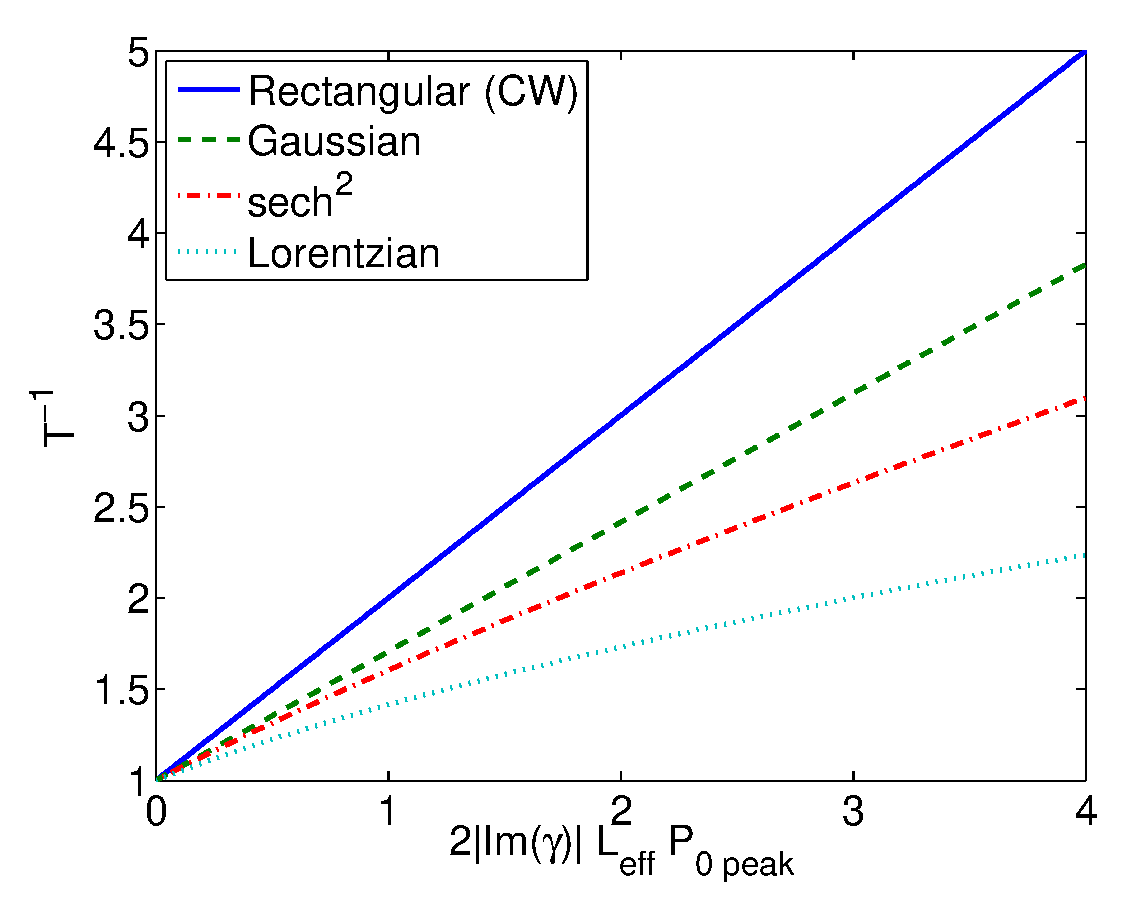
\includegraphics[width=0.5\textwidth]{imGamma_transmissionGaussianLorentzianHypSecant}
    \caption{Absorption simulation for the same averaged power assuming different pulse shapes. As we increase the input power ($P_0$) the transmission can be 5 times smaller than the linear loss.}
    \label{fig:transmissionGaussianLorentzianHypSecant}
\end{figure}


As we can see in Figure~\ref{fig:transmissionGaussianLorentzianHypSecant}, the CW case, which is equivalent to a pulse with a rectangular shape, has a linear dependence with the peak power, while the other shapes are all sub-linear, being the Lorentzian case the most sub-linear. The Gaussian and hyperbolic secant are quite similar.
Instead of using the exact equations shown here, some of which are a bit complicated, one can do an approximation for small $ \delta $:


\begin{equation}
  \tilde{T}^{-1}_{NL~Lorentzian}   = 1 + \frac{1}{2}\delta + O(\delta^2)
  \end{equation}
  
  \begin{equation}
 \tilde{T}^{-1}_{NL~Gaussian}  = 1 + \frac{2}{3}\delta + O(\delta^2) \\
 \end{equation}
 
 \begin{equation}
 \tilde{T}^{-1}_{NL~Hyp.~secant}  = 1 + \frac{1}{\sqrt{2}}\delta + O(\delta^2)
\end{equation}


where $ \delta = 2|Im(\gamma)| L_{eff} P_{0 peak} $. It is worth noting that the slopes are significantly different.


We measure the nonlinear loss coefficient ($|Im(\gamma)|$) using a 1~picosecond laser, a power meter and a variable attenuator (Fig.~\ref{fig:imGammaSetup}). As the shape of the pulses was $sech^2$, we extract $|Im(\gamma)|$ from the fit to equation~\ref{eq:transmissionHypSecantImGamma} after measuring the transmission for different input powers.

\begin{figure}[htb]
    \centering
    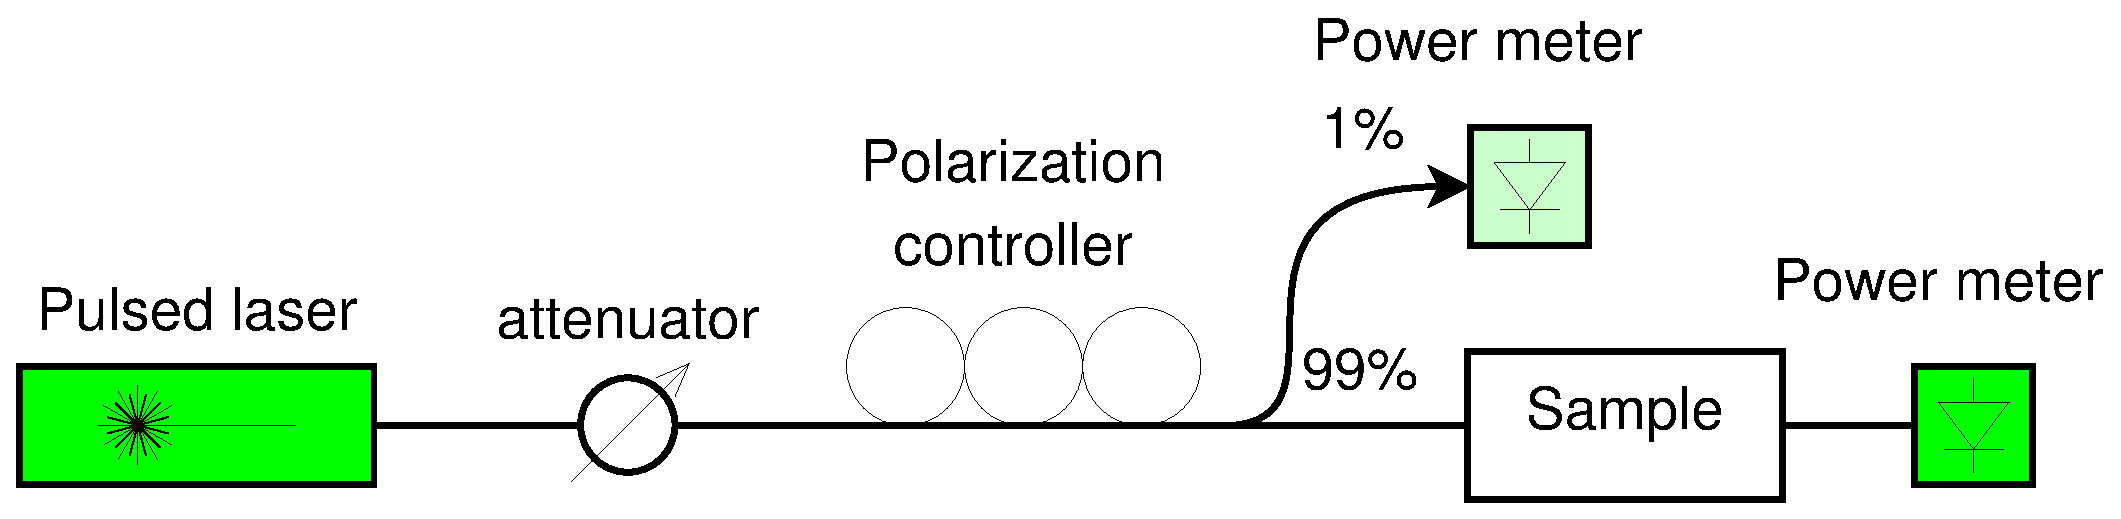
\includegraphics[width=0.80\textwidth]{imGammaFit}
    \caption{We can extract the nonlinear loss coefficient ($|Im(\gamma)|$) from the transmission at different input powers. As we increase the input power, the nonlinear TPA absorption lowers the transmission.}
    \label{fig:imGammaSetup}
\end{figure}


\section{Phase characterization}
\label{ch:phaseCharacterizationSetup}
One of the key parameters in the performance of highly nonlinear devices is group index and chromatic dispersion.
Needless to say that if we want an interaction between two signals with different wavelengths, waveguides should have low dispersion in order to keep this interaction during the longest possible effective length.
Dispersion can be extracted from the phase measurements  modifying slightly the phase sensitive setup that we used for time resolved measurements~\ref{ch:timeRes}.
Phase measurements can also be useful when characterizing the scattering parameters of other optical devices, such as ring resonators, and measuring the group index in slow light structures such as corrugated waveguides.

The phase sensitive experimental setup is a fiber-based MZI, where acousto-optic modulators (AOM) act as frequency shifters (Fig.~\ref{fig:dispersionSetup}).
Each branch applies a slightly different frequency shift (40~kHz in our experiment) and the lock-in amplifier measures the 40~kHz beating pattern.
The phase of these beatings with respect to the RF generators provides the phase of the system, but they are affected by thermal phase noise as high as several radians per second. 
This noise would make unfeasible a phase characterization using a laser with few nm/s tuning speed.
To cancel the phase noise, we introduce from the opposite end a reference counter-propagating beam at a fixed wavelength.
This signal produces another beating pattern used as a reference for the lock-in amplifier.
As thermal fluctuations equally affect both beams, they cancel out, measuring only the wavelength-dependent phase variations.

\begin{figure}[htb]
	\centering
	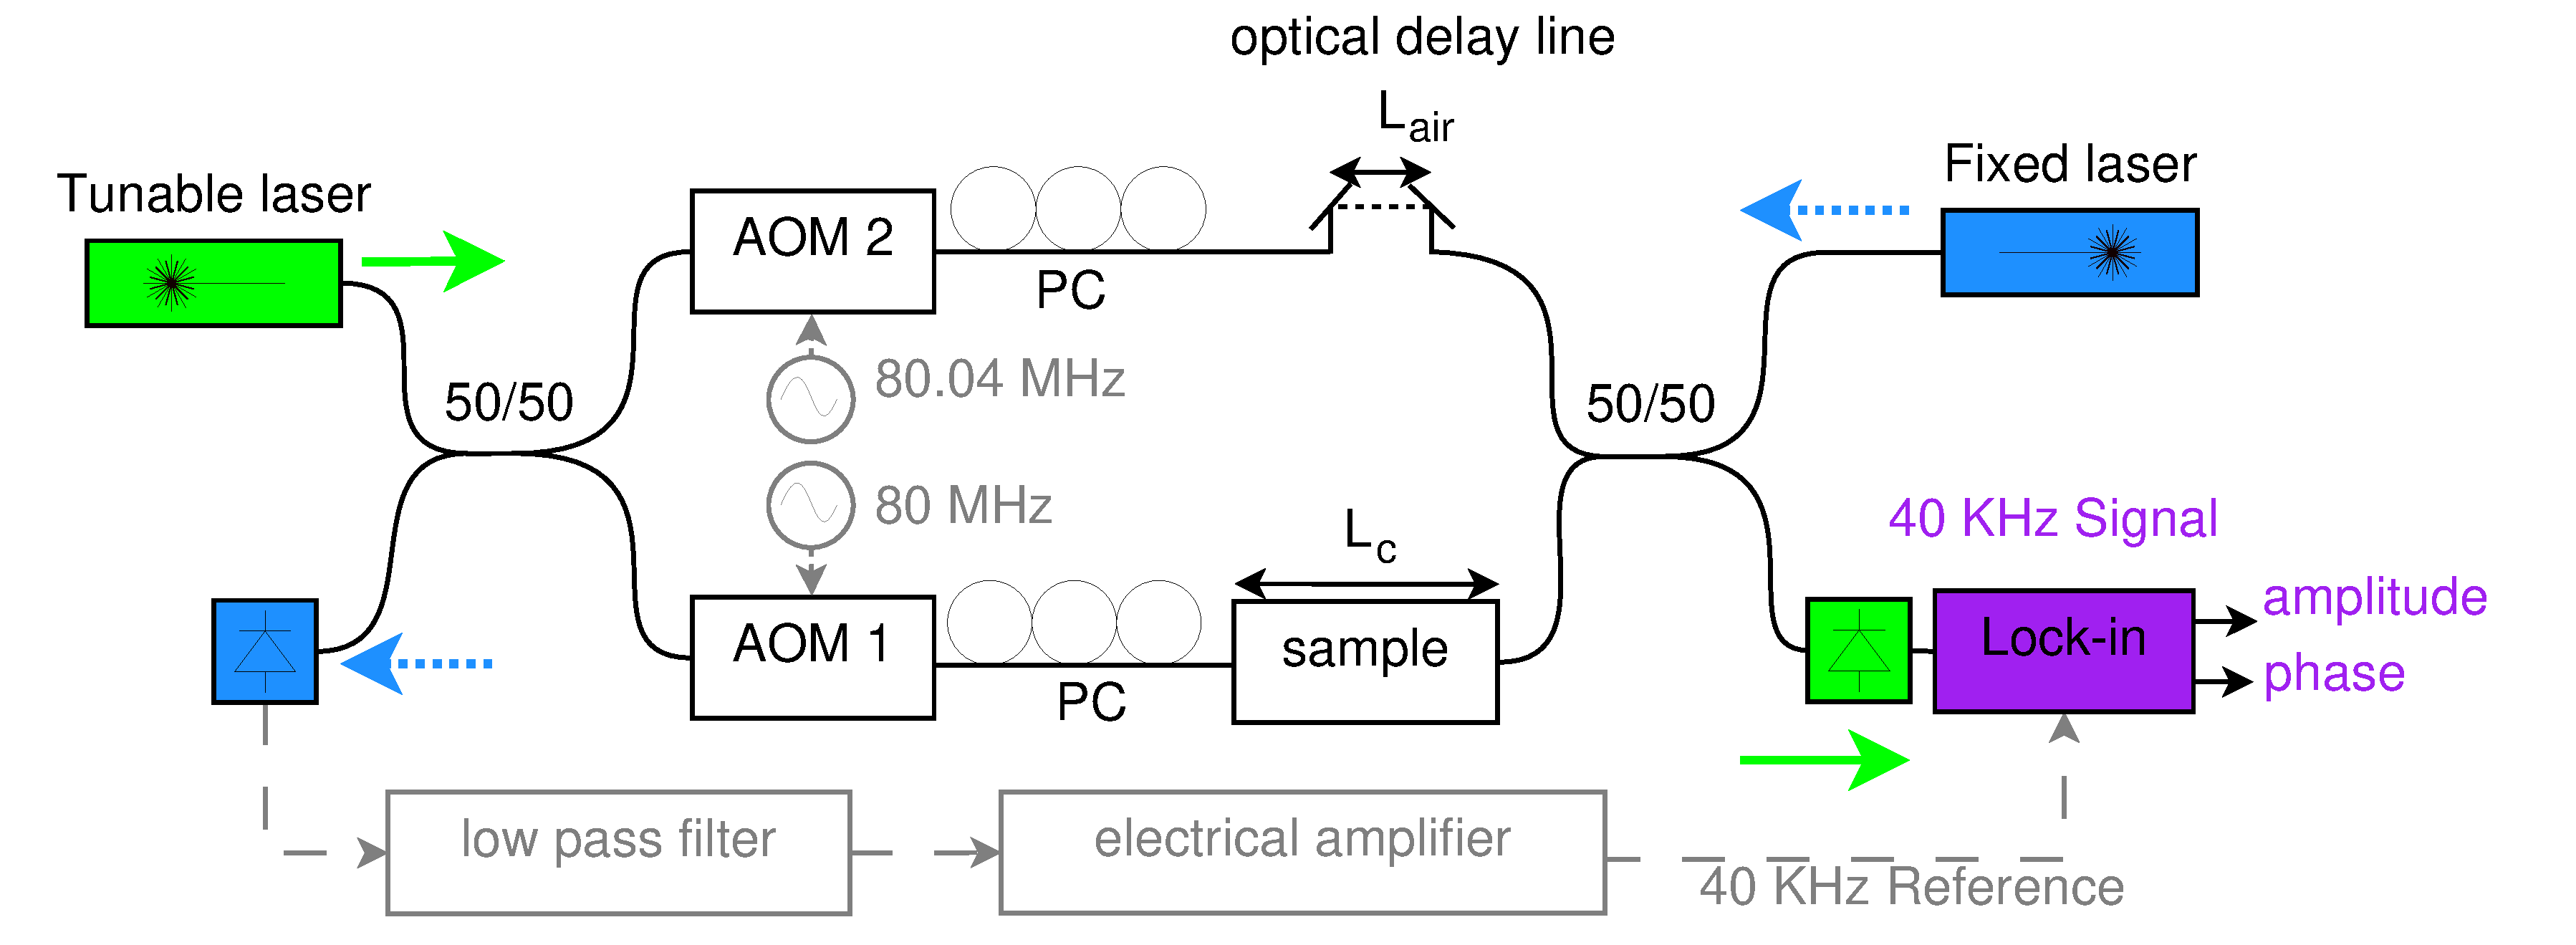
\includegraphics[width=1.00\textwidth]{dispersion6}
	\caption{The lock-in monitors the 40~KHz-beatings using a counter-propagating beam as a reference signal to compensate thermal fluctuations.
	AOM: acousto-optic modulator, PC: polarization controller. }
	\label{fig:dispersionSetup}
\end{figure}


To balance the interferometer for different device lengths there is an optical delay line in the branch without sample.
Before each sweep is launched, the MZI must be balanced in order to avoid too steep slopes in the $\omega$ phase dependence.
In addition, it is convenient to set the wavelength of the counter-propagating reference beam, $\omega_0$, approximately in the middle of the sweep in order to get small phase noise.
If the building block to characterize is in series with other elements, (couplers, connecting waveguides, tapers, etc.) the measurement requires a reference sample with the same elements, but without the component under test (e.g. the corrugated waveguide).
The reference sweep provides the system response, which must be subtracted from the measurement with the component under test. 
Mathematically, the phase dependence obtained with the lock-in, after subtracting the system response, becomes:


\begin{equation}
  \phi(\omega)= \beta_c L_c - \beta_{air} \Delta L_{air} =\phi_{c}(\omega)-\frac{\omega\Delta L_{air}}{c}
  \label{eq:response}
\end{equation}

where $\phi$ is the measured phase, $\phi_{c}$ the phase introduced by the component under test, $\Delta L_{air}$ the extra length introduced in the optical delay line to balance the MZI with respect to the reference measurement, $\beta_c$ and $\beta_{air}$ the propagation constants of the component and of air respectively, and $c$ the speed of light in vacuum.
In Ref.~\cite{Mas2012} we demonstrated that if the component under test has a length $L_{c}$, then the the group index of the component is:

\begin{equation}
  n_{g} = \frac{\Delta L_{air}}{L_{c}}
  \label{eq:group_index_pathBalancing}
\end{equation}

Minimizing the phase versus wavelength slope balances the MZI.
A slope equal to zero at a certain wavelength corresponds to perfect balancing, so one can extract the group index of the component under test.
Finally, from the group index slope variation we extract its wavelength dependence (Section \ref{sec:corrWaveguides}).
It is worth mentioning that the lock-in simultaneously characterizes phase and amplitude in one single sweep.
Moreover, noise due to gradual slight misalignment cancels out normalizing with the amplitude of the reference signal.

Dispersion measurements using setup shown in Fig.~\ref{fig:dispersionSetup} were demonstrated in paper~\cite{Mas2012}.
In one branch of the Interferometer we have the propagation constant of the sample $\beta_s$:

\begin{equation}
	\phi_{s}(\Delta \omega)=  L_{s} \beta_{s}(\Delta \omega)  = L_{s} n_{eff}(\Delta \omega)\frac{\Delta \omega}{c} = L_{s} (\beta_0+\beta_1\Delta \omega+\frac{1}{2!}\beta_2\Delta \omega^2 + \ldots)
\end{equation}

Whereas, in the other branch, we have $L_a$ air propagation in the delay line (ODL) for balancing the interferometer at $\omega_0$ :

\begin{equation}
	\phi_{a}(\Delta \omega)=  \beta_{a}(\Delta \omega) L_{a} =\frac{\Delta \omega}{c} L_{a} 
\end{equation}


To do so we canceled the slope at $\omega_0$ in the $\Delta \omega$ term of the phase evolution:

\begin{equation}
	\Delta \phi = \phi_{s}-\phi_{a}= L_s \beta_0 + \overbrace{ (L_s\beta_1-\frac{L_a}{c})\Delta \omega }+\frac{L_s}{2!}\beta_2\Delta \omega^2 + \ldots)
\end{equation}

From this equalization ($ L_s\beta_1=\frac{L_{a}}{c}$) we can extract the group index from the $\beta_1=n_g/c$ coefficient as:

\begin{equation}
	 n_g=c \beta_1=\frac{L_a}{L_s}
\end{equation}


Being able to extract the dispersion coefficients as:

\begin{equation}
  \beta_i=\frac{d^i\beta}{d\omega^i}\bigg|_{\omega=\omega_0}
\end{equation}


Where $\beta_1$ is related to the group delay and $\beta_2$ defined as the group velocity dispersion (GVD).

\begin{equation}
  \beta_0=\frac{\omega_0}{c} n_{eff}(\omega_0) \,\,\,\,\,  \beta_1=\frac{n_g(\omega_0)}{c} \,\,\,\,\, \beta_2=\frac{-\lambda^2}{2\pi c}D_\lambda
\end{equation}



\begin{figure}[htb]
	\centering
	\includegraphics[width=1.00\textwidth]{dispersionV740}
	\caption{From the phase evolution we can extract the Dispersion of TE and TM strip waveguides with $450 \times 220$ and $500 \times 220$~nm.}
	\label{fig:dispersionMeasurements}
\end{figure}


\section{Optical vector analyzer}
\label{ch:method}
Using a setup similar to the one described in \cite{Vanwiggeren2003} and \cite{Gifford2005} we can also sweep very fast the amplitude and phase spectra of the devices, as the ones shown in chapter~\ref{ch:PhotonicCircuits}. The setup is shown in Fig.~\ref{fig:ovnaSetup} and uses swept-wavelength interferometry (SWI) to measure the complex Jones Matrix of a device. A tunable laser source is in mode-hop free operation capable of sweeping at 1200~nm/s from 1520 to 1620~nm. The sample is in one branch of a Mach-Zehnder interferometer. The output of the interferometer is sent to a $2 \times 2$ coupler, so in one of the photodiodes we receive:

\begin{equation}
	|H(\omega)+je^{-j\omega t}|^2
\end{equation} 


while in the other:

\begin{equation}
	|jH(\omega)+e^{-j\omega t}|^2
\end{equation} 


As it is balance detected the common part of the modulus $|H(\omega)|^2 + 1$ cancels and the remaining is $2j{H}(\omega)e^{j\omega t}+2j\bar{H}(\omega)e^{-j\omega t}$, where $H(\omega)$ is shifted in frequency in one direction and its conjugated $\bar{H}(\omega)$ shifted in the opposite. Finally bandpass filtering the response around $\omega$ we obtain $H(\omega)$.


\begin{equation}
	|H(\omega)+je^{-j\omega t}|^2 - |jH(\omega)+e^{-j\omega t}|^2 = 2j{H}(\omega)e^{j\omega t}+2j\bar{H}(\omega)e^{-j\omega t}
\end{equation} 

\begin{figure}[htb]
    \centering
    \includegraphics[width=0.8\textwidth]{ovna}
    \caption{Optical vector network analyzer schematic.}
    \label{fig:ovnaSetup}
\end{figure}


The optical vector analyzer obtains in real time (1200~nm/s sweeps) impulse responses and amplitude-phase transfer functions. As the sweeps are so fast it can be used for chip alignment and the measurements are immune to thermal fluctuations, time misalignments and other noise sources. It can measure polarization mode dispersion, chromatic dispersion, group delay, insertion losses and amplitude-phase transfer functions for wavelengths from 1520 to 1620~nm. The impulse response in the time domain can be derived form the transfer function and complements perfectly the spectral response of the devices. I used this setup during my stay at the University of California Davis but not in Valencia, so in order to measure the phase response we developed an alternative setup that does not require a very fast sweeping laser (paper~\ref{ch:paperPhase} and section~\ref{ch:phaseCharacterizationSetup}). The commercial version of the setup is the Optical Vector Analyzer of Luna Inc Technologies~\texttrademark .


\pagestyle{plain}
\bibliographystyle{unsrt}
\bibliography{library}
